\section{Evaluation}

\ref{fig:kf-gp-1}, \ref{fig:kf-gp-2}, \ref{fig:kf-gp-3} shows the comparison of the Kalman filter with linear and non-linear model, which we call KF (left) and GP-UKF (right). Under projection, vehicles moving towards the right of the frame has an increasing rate of size and velocity. 
In \ref{fig:kf-gp-1}, tracking just started. GP-UKF tracker does not have any training data, which works similarly with the KF tracker. 
In \ref{fig:kf-gp-2}, GP-UKF has accumulated 1-2 trajectories, showing a slightly better coverage of the actual vehicle. 
Finally, when GP-UKF has 5-8 trajectories as the training data, GP-UFK adapts to the scale and velocity significantly better than linear KF tracker in \ref{fig:kf-gp-3}.

\begin{figure}
\centering
    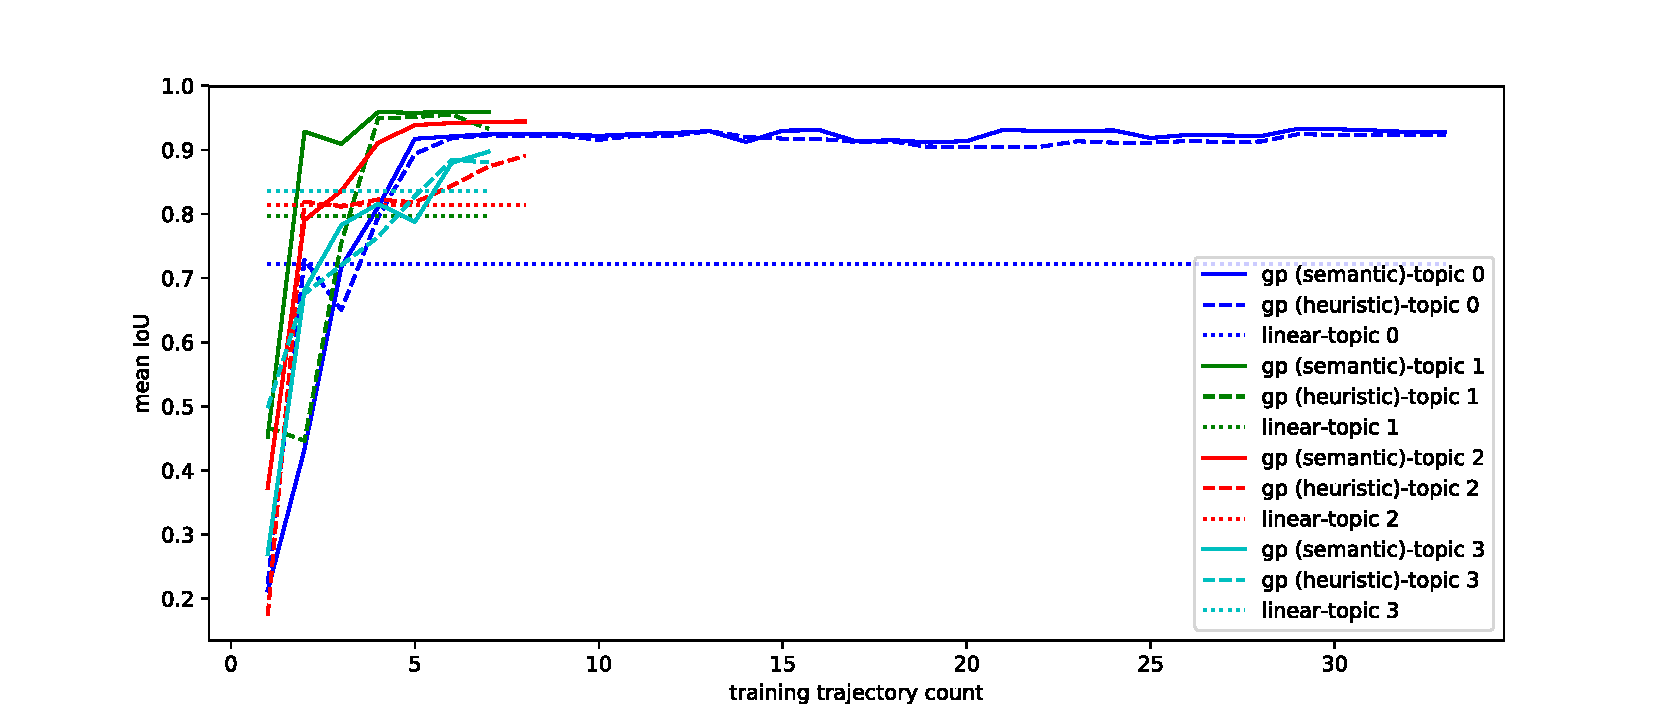
\includegraphics[width=\linewidth]{./img/gp/gp-iou.pdf}
    \caption{The mean IoU of \gls{gp}s trained on the trajectories from the heuristic and semantic tracker, and the linear Kalman filter. Each topic has two \gls{gp}s and a linear Kalman filter.}
    \label{fig:gp-iou}
\end{figure}